\documentclass{standalone}
\usepackage{tikz}
\usetikzlibrary{patterns, positioning}

\begin{document}
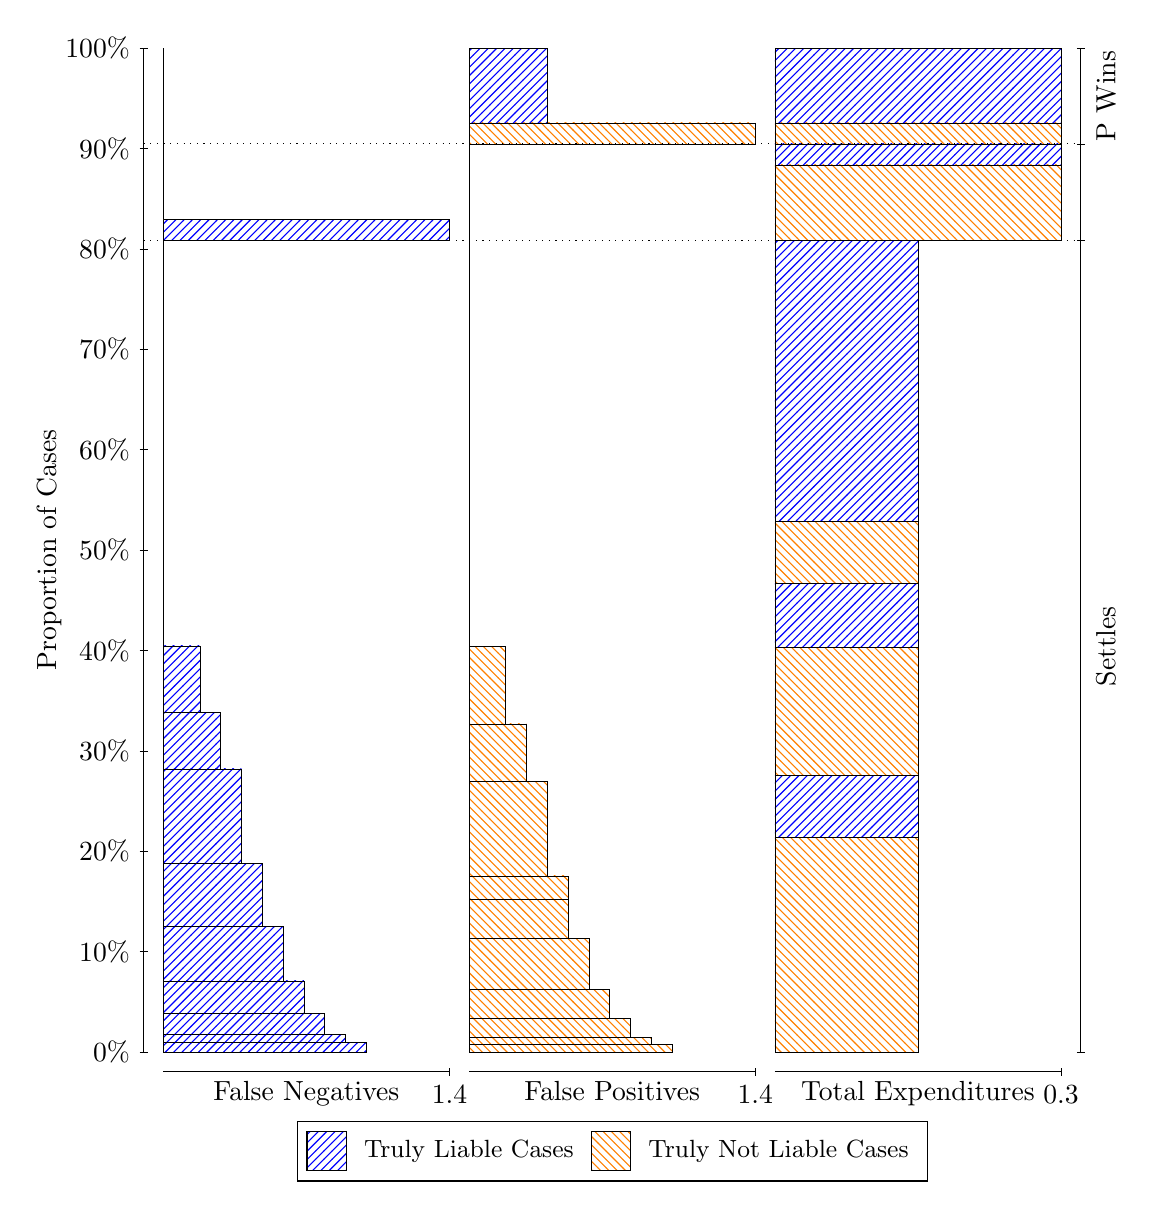
\begin{tikzpicture}
\draw[black, very thin] (1.5,1.75) -- (1.5,14.5);
\node[rotate=90, anchor=center] at (0.3, 8.125) {Proportion of Cases};
\draw[black, very thin] (1.45,1.75) -- (1.55,1.75);
\node[anchor=east] at (1.45, 1.75) {0\%};
\draw[black, very thin] (1.45,3.025) -- (1.55,3.025);
\node[anchor=east] at (1.45, 3.025) {10\%};
\draw[black, very thin] (1.45,4.3) -- (1.55,4.3);
\node[anchor=east] at (1.45, 4.3) {20\%};
\draw[black, very thin] (1.45,5.575) -- (1.55,5.575);
\node[anchor=east] at (1.45, 5.575) {30\%};
\draw[black, very thin] (1.45,6.85) -- (1.55,6.85);
\node[anchor=east] at (1.45, 6.85) {40\%};
\draw[black, very thin] (1.45,8.125) -- (1.55,8.125);
\node[anchor=east] at (1.45, 8.125) {50\%};
\draw[black, very thin] (1.45,9.4) -- (1.55,9.4);
\node[anchor=east] at (1.45, 9.4) {60\%};
\draw[black, very thin] (1.45,10.675) -- (1.55,10.675);
\node[anchor=east] at (1.45, 10.675) {70\%};
\draw[black, very thin] (1.45,11.95) -- (1.55,11.95);
\node[anchor=east] at (1.45, 11.95) {80\%};
\draw[black, very thin] (1.45,13.225) -- (1.55,13.225);
\node[anchor=east] at (1.45, 13.225) {90\%};
\draw[black, very thin] (1.45,14.5) -- (1.55,14.5);
\node[anchor=east] at (1.45, 14.5) {100\%};

\draw[black, very thin] (13.4,1.75) -- (13.4,14.5);
\draw[black, very thin] (13.35,1.75) -- (13.45,1.75);
\node[anchor=west] at (13.35, 1.75) {};
\draw[black, very thin] (13.35,12.054) -- (13.45,12.054);
\node[anchor=west] at (13.35, 12.054) {};
\draw[black, very thin] (13.35,13.283) -- (13.45,13.283);
\node[anchor=west] at (13.35, 13.283) {};
\draw[black, very thin] (13.35,14.5) -- (13.45,14.5);
\node[anchor=west] at (13.35, 14.5) {};

\draw[black, very thin, pattern color=blue, pattern=north east lines] (1.75,1.75) rectangle (4.3264,1.8734);
\draw[black, very thin, pattern color=blue, pattern=north east lines] (1.75,1.8734) rectangle (4.0621,1.9707);
\draw[black, very thin, pattern color=blue, pattern=north east lines] (1.75,1.9707) rectangle (3.7979,2.2372);
\draw[black, very thin, pattern color=blue, pattern=north east lines] (1.75,2.2372) rectangle (3.5336,2.6537);
\draw[black, very thin, pattern color=blue, pattern=north east lines] (1.75,2.6537) rectangle (3.2694,3.3455);
\draw[black, very thin, pattern color=blue, pattern=north east lines] (1.75,3.3455) rectangle (3.0052,4.1468);
\draw[black, very thin, pattern color=blue, pattern=north east lines] (1.75,4.1468) rectangle (2.7409,5.3459);
\draw[black, very thin, pattern color=blue, pattern=north east lines] (1.75,5.3459) rectangle (2.4767,6.0606);
\draw[black, very thin, pattern color=blue, pattern=north east lines] (1.75,6.0606) rectangle (2.2124,6.9075);
\draw[black, very thin, pattern color=orange, pattern=north west lines] (1.75,6.9075) rectangle (1.75,12.054);
\draw[black, very thin, pattern color=blue, pattern=north east lines] (1.75,12.054) rectangle (5.3833,12.321);
\draw[black, very thin, pattern color=orange, pattern=north west lines] (1.75,12.321) rectangle (1.75,13.283);
\draw[black, very thin, pattern color=orange, pattern=north west lines] (1.75,13.283) rectangle (1.75,13.549);
\draw[black, very thin, pattern color=blue, pattern=north east lines] (1.75,13.549) rectangle (1.75,14.5);
\draw[black, very thin, pattern color=orange, pattern=north west lines] (5.6333,1.75) rectangle (8.2097,1.8486);
\draw[black, very thin, pattern color=orange, pattern=north west lines] (5.6333,1.8486) rectangle (7.9455,1.9393);
\draw[black, very thin, pattern color=orange, pattern=north west lines] (5.6333,1.9393) rectangle (7.6812,2.1761);
\draw[black, very thin, pattern color=orange, pattern=north west lines] (5.6333,2.1761) rectangle (7.417,2.5405);
\draw[black, very thin, pattern color=orange, pattern=north west lines] (5.6333,2.5405) rectangle (7.1527,3.1877);
\draw[black, very thin, pattern color=orange, pattern=north west lines] (5.6333,3.1877) rectangle (6.8885,3.6922);
\draw[black, very thin, pattern color=orange, pattern=north west lines] (5.6333,3.6922) rectangle (6.8885,3.9863);
\draw[black, very thin, pattern color=orange, pattern=north west lines] (5.6333,3.9863) rectangle (6.6242,5.1819);
\draw[black, very thin, pattern color=orange, pattern=north west lines] (5.6333,5.1819) rectangle (6.36,5.9162);
\draw[black, very thin, pattern color=orange, pattern=north west lines] (5.6333,5.9162) rectangle (6.0958,6.8963);
\draw[black, very thin, pattern color=blue, pattern=north east lines] (5.6333,6.8963) rectangle (5.6333,12.054);
\draw[black, very thin, pattern color=orange, pattern=north west lines] (5.6333,12.054) rectangle (5.6333,13.016);
\draw[black, very thin, pattern color=blue, pattern=north east lines] (5.6333,13.016) rectangle (5.6333,13.283);
\draw[black, very thin, pattern color=orange, pattern=north west lines] (5.6333,13.283) rectangle (9.2667,13.549);
\draw[black, very thin, pattern color=blue, pattern=north east lines] (5.6333,13.549) rectangle (6.6242,14.5);
\draw[black, very thin, pattern color=orange, pattern=north west lines] (9.5167,1.75) rectangle (11.333,4.4785);
\draw[black, very thin, pattern color=blue, pattern=north east lines] (9.5167,4.4785) rectangle (11.333,5.2589);
\draw[black, very thin, pattern color=orange, pattern=north west lines] (9.5167,5.2589) rectangle (11.333,6.8861);
\draw[black, very thin, pattern color=blue, pattern=north east lines] (9.5167,6.8861) rectangle (11.333,7.7013);
\draw[black, very thin, pattern color=orange, pattern=north west lines] (9.5167,7.7013) rectangle (11.333,8.4918);
\draw[black, very thin, pattern color=blue, pattern=north east lines] (9.5167,8.4918) rectangle (11.333,12.054);
\draw[black, very thin, pattern color=orange, pattern=north west lines] (9.5167,12.054) rectangle (13.15,13.016);
\draw[black, very thin, pattern color=blue, pattern=north east lines] (9.5167,13.016) rectangle (13.15,13.283);
\draw[black, very thin, pattern color=orange, pattern=north west lines] (9.5167,13.283) rectangle (13.15,13.549);
\draw[black, very thin, pattern color=blue, pattern=north east lines] (9.5167,13.549) rectangle (13.15,14.5);
\draw[black, dotted] (1.5,12.054) -- (13.4,12.054);
\draw[black, dotted] (1.5,13.283) -- (13.4,13.283);
\draw[black, very thin] (1.75,1.5) -- (5.3833,1.5);
\node[anchor=north] at (3.5667, 1.5) {False Negatives};
\draw[black, very thin] (5.3833,1.45) -- (5.3833,1.55);
\node[anchor=north] at (5.3833, 1.45) {1.4};

\draw[black, very thin] (5.6333,1.5) -- (9.2667,1.5);
\node[anchor=north] at (7.45, 1.5) {False Positives};
\draw[black, very thin] (9.2667,1.45) -- (9.2667,1.55);
\node[anchor=north] at (9.2667, 1.45) {1.4};

\draw[black, very thin] (9.5167,1.5) -- (13.15,1.5);
\node[anchor=north] at (11.333, 1.5) {Total Expenditures};
\draw[black, very thin] (13.15,1.45) -- (13.15,1.55);
\node[anchor=north] at (13.15, 1.45) {0.3};

\node[black, centered, rotate=90] at (13.72, 6.9019) {Settles};

\node[black, centered, rotate=90] at (13.72, 13.891) {P Wins};

\draw (7.449999999999999,1.5) node[draw=none] (baseCoordinate) {};
\begin{scope}[align=center]
        \matrix[scale=0.5, draw=black, below=0.5cm of baseCoordinate, nodes={draw}, column sep=0.1cm]{
            \node[rectangle, draw, minimum width=0.5cm, minimum height=0.5cm, pattern=north east lines, pattern color=blue] {}; &
            \node[draw=none, font=\small] (B) {Truly Liable Cases}; &
            \node[rectangle, draw, minimum width=0.5cm, minimum height=0.5cm, pattern=north west lines, pattern color=orange] {}; &
            \node[draw=none, font=\small] (B) {Truly Not Liable Cases}; \\
            };
\end{scope}

\end{tikzpicture}
\end{document}